The previous two chapters focused primarily on the performance aspects of task graph execution, by
examining various task scheduling algorithms and also bottlenecks that can limit the scalability of
existing task runtimes. Performance is naturally crucial for \gls{hpc}, yet it should
not be the only factor to focus on. \Autoref{ch:sota} has discussed several other challenges
that affect \gls{hpc} task graphs, that are related to the second main focus of this
thesis, namely the \emph{ergonomics} of task graph execution.

This is a very broad term that encompasses several areas, such as providing an easy way to define
the structure of the task graph, allowing its execution it in an effortless manner (regardless
whether it is on a local computer or a distributed cluster), handling fault tolerance without the
user's intervention, allowing users to express complex resource requirements and many others. This
thesis primarily focuses on analyzing and resolving ergonomical challenges that form a barrier for
executing task graphs on \gls{hpc} clusters.

%While existing task runtimes are able to deal with some of the mentioned challenges with varying
%degrees of success, a unified, dedicated and \gls{hpc}-tailored approach for executing
%task graphs could provide added value to workflow authors, both in terms of ergonomics and
%performance.

%Apart from efficiency, there are several other important challenges have been discussed in. These
%fall under the umbrella of \emph{ergonomics} of task graph execution, which is the second
%primary focus of this thesis. Ergonomics and developer experience in general sometimes tends to be
%neglected in \gls{hpc} applications and tools, which can be notoriously difficult to
%deploy, configure and use.

%While using off-the-shelf task runtimes with \gls{hpc} clusters is possible, these
%tools are not prepared to deal with the idiosyncracies and complexities of supercomputing systems.

%Executing task graphs on \gls{hpc} clusters does not \emph{need} to be
%difficult though, if we use specialized approaches, rather than off-the-shelf tools that are not
%prepared to deal with the complexities of \gls{hpc} systems.

%Furthermore, ergonomics and performance do not
%have to contradict each other -- as we will see in this chapter, approaches that increase
%ergonomics can also help with improving performance and hardware utilization.

One approach to improve ergonomics could be to make incremental improvements to the various
mentioned challenges in off-the-shelf task runtimes. However, as we will see later in this chapter,
ergonomical areas such as supporting heterogeneous tasks and clusters and resource requirements,
providing fault tolerance and dynamic load balancing and overcoming allocation manager limits are
all intertwined, and they affect each other in non-trivial ways. Therefore, this chapter introduces
a holistic meta-scheduling design that aims to tackle the most important challenges with a unified
solution, in order to enable effortless, efficient and fault-tolerant execution of task graphs on
heterogeneous \gls{hpc} clusters in the presence of allocation managers.

This reference design has been implemented in \hyperqueue{}, an
\gls{hpc}-tailored task runtime that was designed to enable transparent, ergonomic and
efficient execution of task graphs on \gls{hpc} systems. \hyperqueue{} is a
spiritual successor of \rsds{}, and builds upon its server and task scheduler
implementation, however it does not use the \dask{} interface. It is the culmination
of the research and work presented in this thesis, which was made possible thanks to the experience
gained from \estee{} and \rsds{}, and also from interacting with many
\gls{hpc} workflows and use-cases over the course of several years.

% TODO: contributions?
%\hyperqueue{} contains the following contributions:
%\begin{enumerate}
%    \item
%\end{enumerate}

%The description of \hyperqueue{}'s implementation and other related concepts in this chapter were
%adapted from our publication~\cite{TODO}.

\workshare{I have collaborated on this work with Ada Böhm, we have both contributed to it equally. I am the sole author of the design and implementation of
specific components of \hyperqueue{}, these will be marked as such in the rest of this chapter. While me and Ada are the primary
contributors to \hyperqueue{}, it should be noted that multiple other people have contributed to it, as its development is a team effort. Source code contribution statistics for \hyperqueue{}
can be found on GitHub\footnoteurl{https://github.com/it4innovations/hyperqueue/graphs/contributors}.}

%First, we will go through the meta-scheduling design, which will be defined in terms of its
%\hyperqueue{} implementation. Then we will examine the implementation details of
%\hyperqueue{}, analyze its performance and evaluate it using several use-cases. Lastly,
%\hyperqueue{} will be compared with other state-of-the-art meta-scheduling task runtimes.

% TODO: rename/restructure


\section{Interaction with allocation managers}
The primary challenge that affects the simplicity of task graph execution on \gls{hpc}
clusters is the presence of an allocation manager, as it forms a barrier; on such clusters, it is
not possible to compute anything at all without interacting with allocations. In order for task
graph execution to become truly ergonomic, there is no point in tackling the rest of the
(ergonomical) challenges until there is a straightforward way of executing task graphs through an
allocation manager.

\Autoref{challenge:allocation-manager} has described several approaches that can be used to map tasks to
allocations, which is necessary to execute task graphs, and also their various shortcomings. Due to
the limits imposed by allocation managers, it might be necessary to partition task graphs into
multiple subgraphs in order to fit them within an allocation, which can be challenging.
Furthermore, it can result in non-optimal usage of hardware resources, because tasks from
(sub)graphs submitted in separate allocations will only be load balanced within their own
allocation, and not across different allocations.

It is important to understand what is uniquely challenging about the interaction with allocations.
The fact that the computation needs to go through a queue is not an issue by itself, as we are
dealing with batch processing anyway. Therefore, some form of a delay between submitting the task
graph and receiving the results is expected, even if we did not have to submit allocations at all.

The main issue of allocations is that they strictly tie together two separate aspects;
\emph{what} does the user want to compute (the computation performed once the allocation
starts) and \emph{where} should the computation take place (specific hardware resources
and computational nodes reserved for the allocation). As was already described previously, both of
these things have to be specified together in an allocation. This is very a inflexible design, for
several reasons:

\begin{itemize}
	\item The user needs to consider both aspects at the same time. Ultimately, the main thing that the user
	      cares about is what do they want to compute. With allocations, they also need to think about
	      specific hardware resources that should be allocated for computing their task graph.
	\item Hardware resources are allocated for the whole duration of the allocation. This can result in
	      inefficient resource usage, especially for heterogeneous task graphs that consist of many types of
	      tasks that use different resources. In situations where not all resources can be used at the same
	      time, some of the resources can unnecessarily sit idle. For example, consider a task graph execuded
	      inside an allocation that provides two computational nodes. Tasks will be load-balanced amongst
	      these two nodes, but towards the end of the computation, there might be tasks that will take a long
	      time to finish. This might lead to a situation where only one of the nodes will be computing the
	      long tail of the remaining tasks, while the second node will be idle. Due to the fact that the
	      allocation cannot release the second node while the computation is still ongoing, the user
	      unnecessarily pays the cost of both nodes until the task graph finishes computing, even though the
	      second node is not doing any useful work.

	\item The amount of used resources has to be decided up front, new hardware resources cannot be added nor
	      removed from existing allocations. This can possibly cause inefficiencies, as described above, but
	      it also limits load balancing. If balancing only happens within (and not across) allocations, users
	      cannot easily provide new hardware resources during the computation, if they realize that it is
	      progressing too slowly.
	\item Granularity of the allocated resources might not match the granularity of tasks. Unless the
	      allocation manager supports very fine-grained allocations (e.g.\ on the level of individual
	      \gls{cpu} cores, rather than whole computational nodes), there can be a large gap
	      between the resources required by a task graph and the resources provided to an individual
	      allocation. This can again lead to resources sitting idle.
	\item Binding computation with specific hardware resources up front complicates fault tolerance. When the
	      user submits thousands of tasks on a specific set of hardware resources, and some of these tasks
	      fail, the user might need to create a new allocation to recompute the failed tasks. This requires
	      figuring out again a new set of hardware resources that should be requested, as the original
	      resources will probably not be a good fit for just a subset of the original computation. A
	      fault-tolerant design would ideally allow recomputing tasks on any compatible hardware resource
	      transparently, which goes against forcing computations and resources to be defined together.
\end{itemize}

It is interesting to note that some of these challenges are uniquely affecting task graphs, and in
general programming models that are different from the traditional ways of defining
\gls{hpc} computations. Consider a distributed application implemented using
\gls{mpi}, which has historically been the most common way of defining computations on
supercomputers. \gls{mpi} applications typically assume that they will run on a set of
computational nodes for a relatively long duration (hours or even days). This set of nodes
(\gls{mpi} processes) usually does not change during the computation; it is not
trivial to add new processes, and if some of the processes crash, it typically leads to the whole
computation being aborted, as fault tolerance is not a default property of \gls{mpi}
applications~\cite{fault_tolerant_mpi}.

These properties of \gls{mpi} applications are similar to the mentioned properties of
allocations, therefore they fit together quite well, and using allocations to execute them is
relatively straightforward. In fact, it is clear that the allocation model itself was designed with
\gls{mpi}-like use-cases in mind. At the same time, it is also not very surprising
that the allocation model is not a good match for programming models that are very different from
\gls{mpi}, such as task-based workflows.

%Note that several of the problems associated with using allocations are directly relevant to
%various challenges from~\Autoref{ch:sota}. Factors such as heterogeneous resource
%requirements, fault tolerance or efficient hardware usage are affected by the usage of allocations.
%Because of that, resolving the problems with allocations should also go a long way towards
%alleviating other ergonomical challenges of task graph execution.


\section{Meta-scheduling design}
This section describes a design for executing task graphs that aims to alleviate the mentioned
challenges by treating task-based programming models as first-class citizens, but still remaining
compatible with allocation managers to enable straightforward execution on \gls{hpc}
clusters. First, we will see a general overview of the design, then we will discuss its properties,
and the following sections will describe its concrete implementation within the
\hyperqueue{} task runtime.

We have seen that the most problematic aspect of allocations is the requirement to define
computations and hardware resources together. The key idea of the proposed design is thus to remove
this property, by completely disentangling the definition of what does the user want to compute
(tasks) from the hardware resources where the computation should take place (computational nodes,
\gls{cpu} cores, etc.). By separating these two concerns, we enable users to focus on
what they care about the most (their task graphs), instead of having to think about mapping tasks
to allocations and graph partitioning.

But how can we disentangle these two concepts, when allocations require us to specify both? The
``trick'' lies in leveraging meta-scheduling on top of allocation managers, which allows us to
change what kind of computation is submitted in allocations and thus simplify the submission
process. The proposed approach is built upon the following three principles.

\begin{description}
	\item[Task runtime runs outside of allocations] Moving the task runtime outside of allocations and running it at some persistent location in the
		cluster (e.g.\ on a login node) enables users to submit tasks to it in a straightforward way and
		crucially also to define the task graph independently of allocations. This removes the need to
		decide which tasks should be computed on which hardware resources and in which allocations up
		front. It can also improve hardware utilization, because it gives the task runtime the ability to
		load balance tasks across all active allocations.

		This is where the term \emph{meta-scheduling} comes in; the essence of the idea is to use a task
		runtime as a sort of high-level scheduler on top of an allocation manager. Instead of forcing users
		to think in terms of allocations, they would be able to submit task graphs in the same way they
		would do it on a system that is not supervised by allocation managers, and let the task runtime
		decide in which allocation should a task be executed in an automatic way.

	\item[Allocations are uniform] Even if the task runtime runs outside an allocation, we still need to submit \emph{some}
		allocations to provide hardware resources that will actually execute tasks. However, instead of
		defining specific tasks that should be computed within an allocation, we can submit allocations
		that execute a generic computational provider (worker), which will connect to the task runtime
		instance running outside the allocation, and then execute any tasks dynamically assigned to it.

		With this approach, allocations become simple and completely uniform, because they all have the
		same structure; each allocation starts a computational provider. This makes it much easier for
		users to submit allocations. Instead of thinking about how to partition their task graphs, users
		simply decide how many computational resources they want to spend at any given moment, and start
		the corresponding number of allocations. Furthermore, this also allows the task runtime to submit
		allocations completely automatically based on computational needs, without the user having to do
		anything manually.
	\item[Pair tasks with workers using abstract resources] The principles described above separate the two core pillars of task graph execution; the
		definition of the task graph and the provisioning of hardware resources. However, we actually do
		need to have \emph{some} way of tying these two concepts together, because tasks might
		have various constraints on the environment in which they can be executed. While using allocations
		directly for submitting tasks provided this binding implicitly, we saw that it also had many
		disadvantages. What we can do instead is to use an abstract resource system. Each task will have a
		set of abstract resources required by it, and each worker will in turn provide a set of abstract
		resources provided by it. The task runtime will then dynamically assign tasks to workers by
		matching these resources together.

		As an example, a task can specify that it requires four \gls{cpu} cores and two
		\glspl{gpu}. If we provide the task runtime with a worker that has 128 cores and 8
		\glspl{gpu}, it could schedule up to four instances of this task on this worker at the
		same time.

		This approach allows defining complex heterogeneous tasks while still allowing users to provide
		workers independently of tasks.
\end{description}

The proposed design enables straightforward execution of large task graphs that contain
dependencies and are heterogeneous, because it sidesteps the allocation manager by moving the task
runtime outside of allocations. This avoids the limits associated with executing tasks in
allocations directly, such as limited support for dependencies, limited scale of task graphs that
can be executed, and non-optimal load balancing and hardware utilization. This scheme also directly
alleviates additional challenges mentioned in~\Autoref{ch:sota}.

Achieving fault tolerance becomes easier, because tasks are no longer tied to specified
allocations. Instead, tasks are stored in a persistent task runtime instance. When a task fails,
the runtime can simply recompute it, even in a different allocation than where it was originally
started. Heterogeneous task graphs can be executed without having to consider allocation limits,
due to the usage of abstract resources. And task scheduling becomes more flexible, since the
runtime can dynamically use resources that are provided by multiple allocations, which can help
with improving hardware utilization.

Of course, this approach is not a panacea, and it also introduces certain trade-offs. Running the
task runtime on a login node might be problematic if the login nodes are severely computationally
constrained or if they are not even able to connect to compute nodes of the \gls{hpc}
cluster through the network. While the runtime could also be executed elsewhere, for example in a
cloud partition of a cluster, or even inside allocations themselves (in that case it would still
communicate with workers running in different allocations), although this would complicate the
deployment process and might require additional resiliency features to be implemented in the task
runtime.

To evaluate how does the proposed approach work in practice, what are its performance and usage
implications and how does it compare to existing meta-schedulers, we have implemented this design
in a task runtime called \hyperqueue{}, which will be described in the rest of this
chapter.

\section{\hyperqueue{}}
\hyperqueue{} is a distributed task runtime that aims to make task graph execution a
first-class concept on supercomputers. It does that by implementing the meta-scheduling design
described in the previous section, and providing functionality optimized for \gls{hpc}
use-cases. In terms of architecture and implementation, it is an evolution of the
\rsds{} task runtime described in~\Autoref{ch:rsds}, however instead of using
the \dask{} components and \glspl{api}, it implements its own task-based
programming model. \hyperqueue{} is developed in the Rust programming language and it is
provided as an \mbox{MIT-licensed} open-source tool~\cite{hq_github}.

This section describes the high-level design of \hyperqueue{}, its most important features
and also how it tackles the challenges mentioned in~\Autoref{ch:sota}. Note that for
simplicity, Slurm will be used as an example of an allocation manager throughout this whole
chapter, but it could be replaced by PBS or any other commonly used allocation manager without the
loss of generality.

\subsection{Architecture}
\hyperqueue{} uses a fairly standard distributed architecture. It consists of three main
components, a central management component called a \emph{server}, a component that serves
as a computational provider which executes tasks, called a \emph{worker}, and an interface
for submitting tasks, called a \emph{client}.~\Autoref{fig:hq-architecture} displays a high-level
view of the \hyperqueue{} architecture for a typical deployment on an
\gls{hpc} cluster with an allocation manager, where the server runs on a login node
and meta-schedules tasks on top of various allocations running on computational nodes. The
individual components are described in more detail below.

\begin{figure}[h]
	\centering
	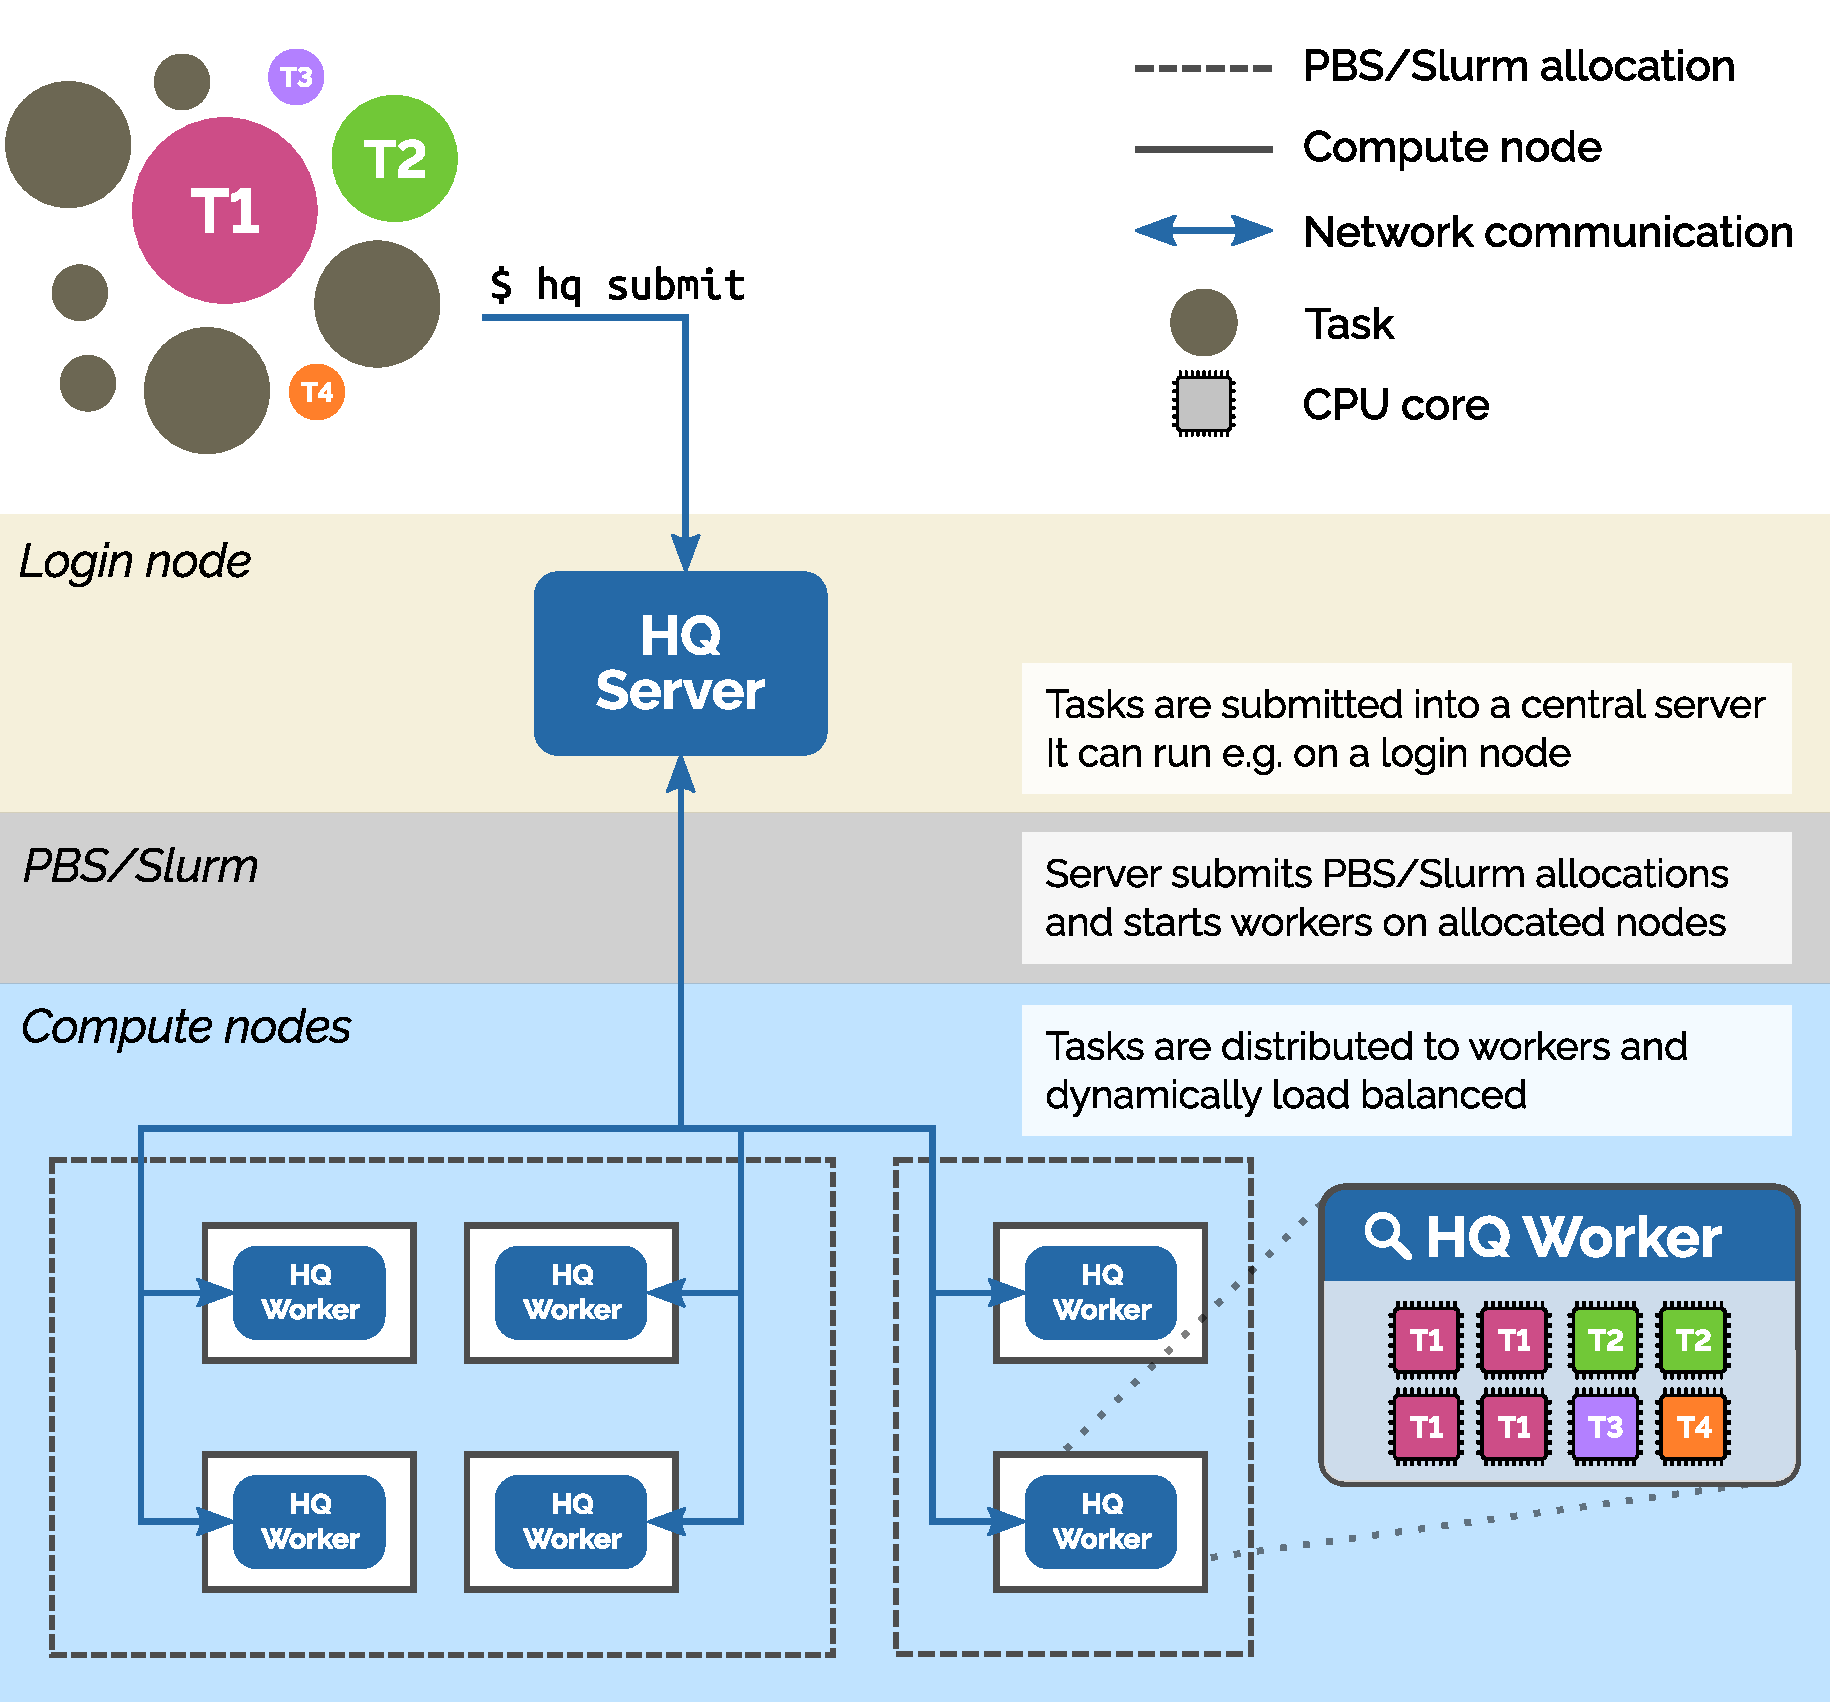
\includegraphics[width=0.9\textwidth]{imgs/hq/architecture}
	\caption{Architecture of \hyperqueue{}.}
	\label{fig:hq-architecture}
\end{figure}

\subsubsection*{Server}
The \emph{server} is the most important part of \hyperqueue{}. Its main goal is
to manage both the lifecycle of task graphs and of workers that provide computational resources. It
keeps track of all tasks and workers, and allows users to query their state and also send commands
to it through a client interface. The server contains a work-stealing task scheduler that is based
on the \rsds{} scheduler implementation described in~\Autoref{sec:rsds-description}. The
scheduler assigns individual tasks to workers based on task resource requirements and current
computational load of workers, in order to maximize hardware utilization.

It is designed to be executed as a long-running background process in a persistent location not
managed by allocation managers (i.e.\ outside ephemeral allocations). Typically, it will be
executed on a login node of a cluster, but it can also run elsewhere, for example in a cloud
partition. It should keep running until all task graphs that the user wants to execute are
finished, although it can also restore its state from disk, so the computation of a task graph can
be interrupted and resumed at a later time.

The fact that the server runs outside allocations allows it to load balance tasks across workers
running in multiple allocations concurrently, and work around the various limits of allocation
managers. This adheres to the first principle of the meta-scheduling design described in the
previous section.

The \hyperqueue{} server itself does not execute any tasks, and it consumes a relatively
modest amount of resources, therefore it is not computationally demanding. Section
TODO\todo{fix link} will evaluate its resource consumption in a typical scenario.

Apart from basic responsibilities related to worker management and task scheduling, the server can
also provide additional functionality, which will be described later in the text.

\subsubsection*{Worker}
The \emph{worker} component is a computational provider that executes tasks assigned to it
by the server. A single worker typically manages all hardware resources (\gls{cpu}
cores, \gls{gpu} or \gls{fpga} accelerators, memory, etc.) of a given
computer, usually a single computational node of a supercomputer.

The worker is able to automatically detect all relevant hardware resources that are available on
the node where it is started and advertise them to the server. Therefore, in the typical case,
users can simply start the worker on a given node with a single uniform command, and from that
moment on the resources of that node will be used for task execution. This adheres to the second
principle of the proposed meta-scheduling design, where computational provides should be generic,
and it should be possible to start them using a uniform command, to make their deployment trivial.

Each worker also participates in task and resource scheduling. The server makes high-level
scheduling decisions, such as which tasks will be executed on a given worker, while the worker then
performs micro decisions, such as in which order will it execute tasks assigned to it, or which
specific resources will be assigned to a given task. Resource management will be described in more
detail in a later section.

An important aspect related to workers is fault tolerance. On an \gls{hpc} cluster,
\hyperqueue{} workers are designed to be executed inside allocations that only run for a
limited amount of time, which implies that they can disappear during the computation of a task
graph, but also that new workers can be added at any time. Both the server and workers thus operate
with the assumption that workers can be potentially short-lived; if a worker disconnects while it
is executing a task, the task will be transparently reassigned to a different worker, without user
intervention. This property also enables users of \hyperqueue{} to arbitrarily scale the
computation of a task graph both up and down, even while it is being executed, by dynamically
adding or removing workers as needed.

While workers can be deployed manually by users, \hyperqueue{} can also automatically
submit allocations to an allocation manager that start workers on computational nodes, based on
current computational needs of submitted task graphs. This system, called \emph{automatic allocation},
will be described in more detail later in Section TODO\todo{link}.

\subsubsection*{Client}
After starting the server, users can start submitting task graphs to it using one of several
interfaces, which implement the \emph{client} component. The client interfaces and the
programming model used by \hyperqueue{} will be described in~\cite{hq:programming-model}.

\subsubsection*{Deployment}
Even though it is often overlooked, deployment of software on supercomputers can be challenging, as
was described in~\Autoref{challenge:deployment}. Since \hyperqueue{} aims to provide seamless
support for \gls{hpc} use-cases, it was also designed to be trivial to deploy. It is
distributed as a single, relatively small (approx. 15 MiB), statically linked executable, which
implements all the provided functionality (server, worker and client components). It does not
depend on any external services or dynamic libraries, apart from the ubiquitous
\texttt{C} standard library, and it runs fully in userspace and does not require any
elevated privileges. It also does not require any installation step nor any configuration to be
used.

Both clients and workers communicate with the server using the standard \gls{tcpip}
protocol, which is ubiquitously available on most clusters. By default, all communication is
encrypted, so that other users of the cluster cannot observe the data sent between the
\hyperqueue{} components. This is performed out of an abundance of caution, because the
server typically runs on a login node, which is shared by multiple users, rather than on
computational nodes, which are usually isolated between users by the allocation manager.

In order to connect the individual components using \gls{tcpip}, normally it would be
required for users to specify network hostnames and ports. While this process is relatively simple,
it still presents a minor ergonomical hurdle, because users would need to reconfigure their worker
deployment scripts and client commands every time the server would start on a new
\gls{tcpip} address. To make this easier, \hyperqueue{} removes the need to
specify hostnames and ports by default, by exploiting a useful property of \gls{hpc}
clusters, which commonly use a shared networked filesystem. When a server is created, it creates a
configuration file in the user's home directory, which contains all information necessary for
exchanging handshakes and connecting the components. When workers and clients discover the presence
of this file (which can be accessed due to the filesystem being shared), they are able to connect
to the server without the user having to specify any addresses.

Thanks to these properties, it is trivial to deploy and use \hyperqueue{} on
supercomputers, even without the involvement of the administrators of the target cluster. The
deployment benefits extend also beyond \gls{hpc} clusters. Users can also trivially
deploy \hyperqueue{} on their own personal computers. This enables them to prototype
their \gls{hpc} workflows locally, which can accelerate their development process and
is another step towards improving the ergonomics of using task graphs on supercomputers. This is in
contrast with using allocation managers for submitting tasks directly, which makes local
experimentation very difficult, as allocation managers are not straightforward to deploy on
personal computers.

\subsection{Programming model}
\label{hq:programming-model}
The programming model used by \hyperqueue{} is optimized for common
\gls{hpc} use-cases.

- it does not support data transfers yet
- iterative computation?
- terminology
- task states
- common workflow

\subsubsection{Interface}
- CLI
- Python API

\subsubsection{Scheduling and resource management}

\subsubsection{Output streaming}

\subsubsection{Multi-node tasks}

\subsection{Automatic submission of allocations}
The meta-scheduling design employed by \hyperqueue{} resolves the most important
challenges associated with allocation managers, and it makes creating allocations simple, so that
users can scale the computational resources used for computing their task graphs
at will. However, creating allocations manually can still be relatively demanding for some users,
who might want to employ a more automated approach for scaling computational resources. Since
\hyperqueue{} knows the state of all tasks and workers, and it is commonly executed on login
nodes that have access to allocation managers, it is also able to automatically submit new
allocations on behalf of the user, based on current computational load. This system, which is called
\emph{Automatic allocator}, will be described in this section.

\workshare{I am the primary author of the design and implementation of the automatic allocation
system in \hyperqueue{}.}



- experiment with hardware utilization

\section{Case study: LiGen}

\section{Case study: GROMACS}

\section{Evaluation}
We have designed a series of experiments that evaluate the performance and scalability of
\hyperqueue{} and also its ability to maximize hardware utilization of workers. All
experiments were performed on the \gls{cpu} partition of the Karolina
supercomputer~\cite{karolina} located at the IT4Innovations supercomputing
center~\cite{it4i}. Each non-accelerated computational node of Karolina has two AMD
EPYC\texttrademark{} 7H12 2.6 GHz 64 core \glspl{cpu}, for a total of 128 cores per
node, and 256 GiB of DDR4 \gls{ram}. It runs on the RockyOS 8 operating system with Linux kernel
$4.18.0$ and \texttt{glibc} (GNU \texttt{C} standard library implementation) $2.28$.

% TODO: all experiments were performed with the 0.1X version of HyperQueue, using commit XYZ.

\subsection{Server \gls{cpu} usage}
The \hyperqueue{} server component is primarily designed to be executed on login nodes when
deployed on supercomputers. This could pose a problem if it consumed too many system resources,
because login nodes are shared by multiple users, and they are not designed for computationally
intensive tasks. Some clusters even forcefully limit the total amount of \gls{cpu}
time that can be consumed by processes running on login nodes~\cite{leonardo_time_limit}, and
terminate the process if it exceeds the maximum allowed time.

\begin{figure}[h]
	\centering
	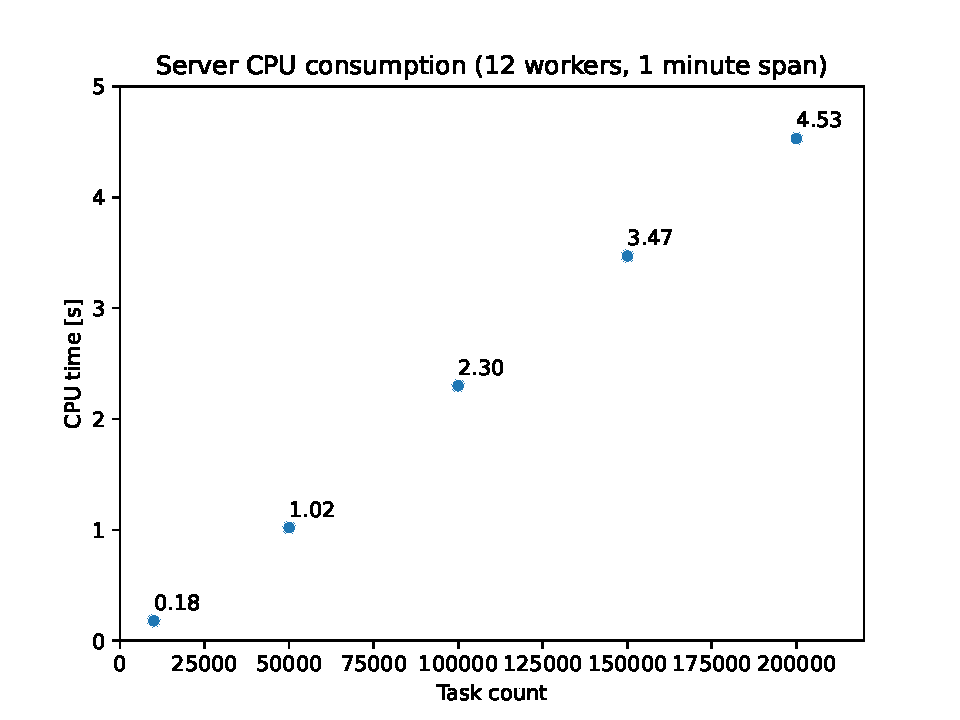
\includegraphics[width=0.7\textwidth]{imgs/hq/charts/server-utilization-tasks}
	\caption{\gls{cpu} time consumption of the \hyperqueue{} server}
	\label{fig:hq-server-cpu-consumption}
\end{figure}

To evaluate how many resources does the server consume, we have performed an experiment on the
Karolina cluster, where the server had to schedule a large amount of tasks in a short time period
(which acts as a stress test), and we measured its total \gls{cpu} time consumption
across all cores.

The server was running on a login node, and it was managing $12$ workers
(therefore $1536$ cores). Each worker was deployed on a computational node in a
separate allocation, so that the server had to communicate with the workers over the network. It
had to schedule an increasing number of tasks (from $10$ to $200$
thousand) over a fixed time span. The duration of each task was scaled so that the whole task graph
would always finish computing in exactly one minute. We measured the total amount of
\gls{cpu} time consumed by the server (both in user-space and in the kernel), using
standard Linux monitors.

We can observe the results of this experiment in~\Autoref{fig:hq-server-cpu-consumption}. The horizontal axis shows
the number of tasks that were used for the given benchmark run, and the vertical axis shows the
\gls{cpu} time consumed by the server over the one-minute period. We can see that the
amount of \gls{cpu} resources scales linearly with the amount of tasks scheduled by
the server. In the worst case, the server has consumed less than five seconds of
\gls{cpu} time over one minute of real time, even though it had to schedule
$200$ thousand tasks within this short period, which is an extreme stress test that
far exceeds the rate of scheduled tasks in most scientific workflows. Over all the benchmarked task
counts, the average \gls{cpu} consumption of the server per second and per
$1000$ tasks was approximately $0.00034$~s. In other words, for every
thousand tasks in the task graph, the server consumed approximately $0.3$~ms
\gls{cpu} time every second.

The amount of used resources will of course vary based on the executed workflow. However, this
experiment shows that the server consumes very few resources in general, and that it still has a
lot of leeway, even if some task graphs proved to be more computationally demanding than the
benchmarked stress test.

% Other benchmarks
- many sleep 0 tasks
- hardware utilization
- task storage optimization?

\section{Comparison with state-of-the-art}
%TODO: Merlin https://merlin.readthedocs.io/en/latest/tutorial/1_introduction/?h=many#how-can-merlin-run-so-many-simulations
%TODO: Balsam https://arxiv.org/abs/1909.08704
%TODO: FireWorks https://onlinelibrary.wiley.com/doi/10.1002/cpe.3505
%TODO: Parsl
%TODO: Dask

\section*{Summary}
This chapter has presented a meta-scheduling design designed for execution of task graphs on
\gls{hpc} clusters that was built from the ground up to overcome the issues mentioned
in\Autoref{ch:sota}. It has also introduced \hyperqueue{}, a distributed task
runtime that implements this design through an \gls{hpc} focused programming model,
which (together with its trivial deployment) makes it easy and ergonomical to run workflows on
supercomputers.  We have performed various performance evaluations% TODO: přepsat
of \hyperqueue{}, which have showed that the server does not consume a lot of resources
and that the tool as a whole is competitive with other similar tools.

\hyperqueue{} has already been adopted in several projects, and it is also being actively
used by researchers and teams across several \gls{hpc} centers. It has been proposed
as one of the designated ways for executing \gls{hpc} computations in several
supercomputing centers and clusters, such as LUMI~\cite{it4i-lumi},
IT4Innovations~\cite{it4i-hq} or CINECA~\cite{cineca}.

In addition to being used directly by users as a task runtime, \hyperqueue{} can also be
used as a task execution system, thanks to its sophisticated resource management and task
scheduling capabilites. It facilitates this use-case by offering a machine-readable
(\gls{json}) output mode for its \gls{cli}, which makes it easier for
other tools to use \hyperqueue{} programmatically. This has been leveraged by several
workflow management systems that have integrated \hyperqueue{} as one of their task
execution backends, such as Aiida~\cite{aiida-hq}, NextFlow~\cite{nextflow-hq},
UM-Bridge~\cite{umbridge} or ERT~\cite{ert}.

\hyperqueue{} is also being used by in various research projects. As an example,
scientists from the Czech Academy of Sciences use it to execute tasks that analyze data from the
ATLAS~\cite{atlas} experiment performed at CERN. In this case, it was able to improve
hardware utilization by 30\%~\cite{cern-hq} on the IT4Innovations \gls{hpc}
cluster. \hyperqueue{} has also been used to execute workflows in several European Union
projects, such as Ligate\cite{ligate}, EVEREST~\cite{everest},
ACROSS~\cite{across} and MaX~\cite{max}.

Given the use-cases mentioned above, I am confident that \hyperqueue{} does provide a
tangible benefit for its users in terms of ergonomical and efficient execution of task graphs on
supercomputers, and that it does alleviate many challenges, that have been extensively in this
thesis, in practice. I hope that \hyperqueue{} will eventually see even more widespread
usage in the \gls{hpc} community.
